\documentclass[11pt,a4paper,oneside]{article}

%\usepackage{pscyr}
\usepackage[T2A]{fontenc}
\usepackage[utf8x]{inputenc}
\usepackage[english,russian]{babel}
\usepackage{expdlist}
\usepackage[dvips]{graphicx}
\usepackage{subcaption}
\usepackage{amsmath}
\usepackage[makeroom]{cancel}
\usepackage{svg}
\usepackage[top=1in, bottom=1in, left=1in, right=1in]{geometry}
\usepackage{indentfirst}
\usepackage{mathtools}

\begin{document}

\begin{center}
	{Вяцков Михаил, КН-401}
	
	{\huge \bf Лабораторная работа №6}
\end{center}

\section{Условия}

Решить следующую краевую задачу на отрезке $[0, 5]$

$$ y'' - y = 0.9 (x^3 - x^2 + 2) $$
$$ y'(0) = -6.4 = \alpha $$
$$ y'(5) = e^5 + 2e^{-5} - 63.9 = \beta $$

Решая задачу аналитически, получаем

$$ y = C_1 e^x + C_2 e^{-x} - 0.9 (x^3 - x^2 + 6x) $$

Осталось найти коэффиценты

$$ y' = C_1 e^x - C_2 e^{-x} - 0.9 (3 x^2 - 2 x + 6) $$

$$ 
\left\{\begin{matrix}
	C_1 - C_2 = -6.4 \\
	C_1 e^5 - C_2 e^{-5} - 0.9 \cdot 71 = e^5 + 2 e^{-5} - 0.9 \cdot 71
\end{matrix}\right.
$$

Найдем численным методом коэффиенты, решив систему уравнений

$$
\left\{\begin{matrix}
	C_1 = 1.00018161 \\
	C_2 = 2.00018161
\end{matrix}\right.
$$

Погрешность решения системы $\pm 5 \cdot 10^9$.

\section{Методы}

\subsection{Стрельбы}

Зафиксируем некоторую неизвестную величину $\mu$ и произведем замену переменных

$$ y(0) = \mu $$
$$ y' = p $$
$$ p' = y + 0.9 (x^3 - x^2 + 2) $$
$$ u = (y, p)^\tau $$
$$ u' = \phi(x, u) = \left(\begin{matrix}
	0 & 1 \\
	1 & 0 \\
\end{matrix}\right) u + (0, 0.9 (x^3 - x^2 + 2))^\tau $$

Перед нами некоторая задача Коши, используя которую надо получить верное условие на второй конец

$$ p(5, \mu) = \beta $$

Решать задачу Коши будет методом Рунге-Куты 3 порядка, а решать нелинейное уравнение методом деления отрезка пополам. В качестве начального значения попробуем брать несколько точек в некотором диапозоне и брать ту, из которой сошлось к ответу быстрее всего (если вообще сошлось).

Конкретнее, возьмем отрезок от -100 до 100 (смелое предположение), и будем сжимать его на 20\% на каждом шаге, пока не сойдемся к корню (или локальному минимуму и тогда будем думать дальше).

Точность данного метода квадратичная, с учетом того, что начальное условие находится с машинной точностью.

\subsection{Разностной прогонки}

Обозначим

$$ y'' = y + 0.9 (x^3 - x^2 + 2) = p(x) y + q(x) $$

Обозначим за $y_i$ приближеное значение функции в узлах $x_i = a + h i$, а также $p_i = p(x_i), q_i = q(x_i)$. Воспользуемся формулой численного дифференцирования по трем узлам на середину во всех узлах, кроме крайних, получим

$$ y''(x_i) \approx p_i y_i + q_i = \frac{y_{i - 1} - 2 y_{i} + y_{i + 1}}{h^2}, i = 1 \dots n - 1 $$
$$ y_{i - 1} - (2 + p_i h^2) y_{i} + y_{i + 1} = q_i h^2 $$

Для крайних узлов воспользуемся формулой численного дифференцирования по двум узлам на правый (левый) узел для первого (последнего) из исходных узлов.

$$ y'(a) \approx \frac{y_1 - y_0}{h} $$
$$ y_1 - y_0 \approx h y'(a) $$
$$ y'(b) \approx \frac{y_n - y_{n - 1}}{h} $$
$$ y_{n - 1} - y_n \approx - h y'(b) $$

Таким образом метод будет иметь первый порядок точности и уравнение для приближенного решения будет выглядить следующим образом

$$\left(\begin{matrix}
	-1      & 1              & 0              & \dots  & 0      & 0      & 0      \\
	1      & -(2 + p_1 h^2) & 1              & \dots  & 0      & 0      & 0      \\
	0      & 1              & -(2 + p_2 h^2) & \dots  & 0      & 0      & 0      \\
	
	\vdots & \vdots         & \vdots         & \ddots & \vdots & \vdots & \vdots \\
	
	0 & 0 & 0 & \dots  & -(2 + p_{n - 2} h^2) & 1                    & 0      \\
	0 & 0 & 0 & \dots  & 1                    & -(2 + p_{n - 1} h^2) & 1      \\
	0 & 0 & 0 & \dots  & 0                    & 1                    & -1      \\
\end{matrix}\right)
\left(\begin{matrix}
	y_0 \\
	y_1 \\
	y_2 \\
	\vdots \\
	y_{n - 2} \\
	y_{n - 1} \\
	y_{n} \\
\end{matrix}\right)
=
\left(\begin{matrix}
	h y'(a) \\
	q_1 h^2 \\
	q_2 h^2 \\
	\vdots \\
	q_{n - 2} h^2 \\
	q_{n - 1} h^2 \\
	- h y'(b) \\
\end{matrix}\right)$$

Остается решить эту систему методом прогонки, чтобы получить результат. Для того, чтобы эффективно использовать метод прогонки, необходимо выполнения условия диагонального преобладания

$$ |a_{ii}| \ge \sum_{i \neq j} |a_{ij}| $$

Причем хотя бы единожды должно выполнятся строгое неравенство. Заметим, что для первого и последнего элементов на диагонали выполняется равенство, а для остальных

$$ |a_{ii}| = 2 + p_i h^2 = 2 + h^2 > 2 = 1 + 1 = \sum_{i \neq j} |a_{ij}| $$

То есть условие диагонального преобладания выполнено.

\pagebreak
\section{Численный эксперимент}

Значение параметра в методе стрельбы получилось примерно равным 3 ($\approx 3.0003436926$).

\begin{figure}[h]
	\begin{subfigure}{0.5\textwidth}
		\centering
		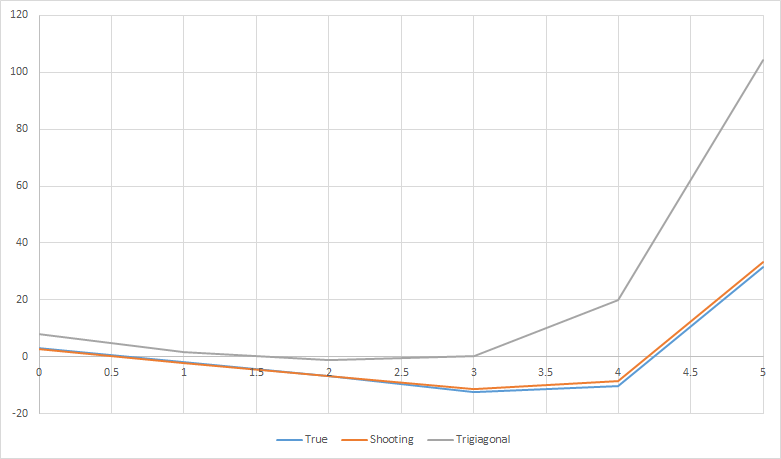
\includegraphics[width=0.9\linewidth]{pics/plot1.png}
		\caption{Шаг $h=1$}
	\end{subfigure}
	\begin{subfigure}{0.5\textwidth}
		\centering
		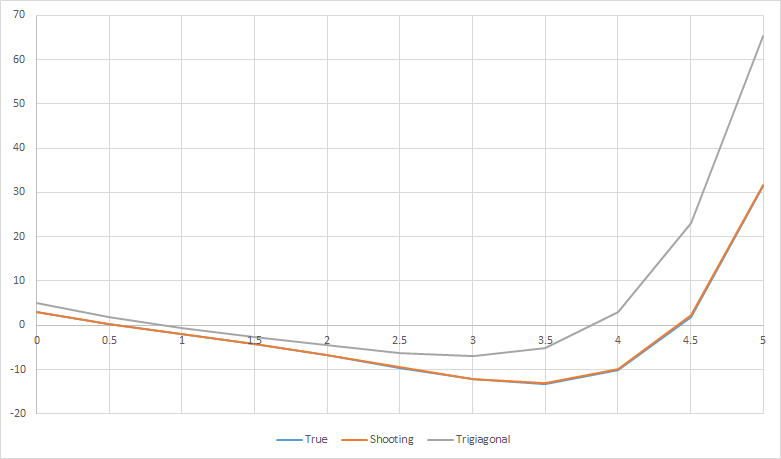
\includegraphics[width=0.9\linewidth]{pics/plot2.png}
		\caption{Шаг $h=0.5$}
	\end{subfigure}
	\begin{subfigure}{0.5\textwidth}
		\centering
		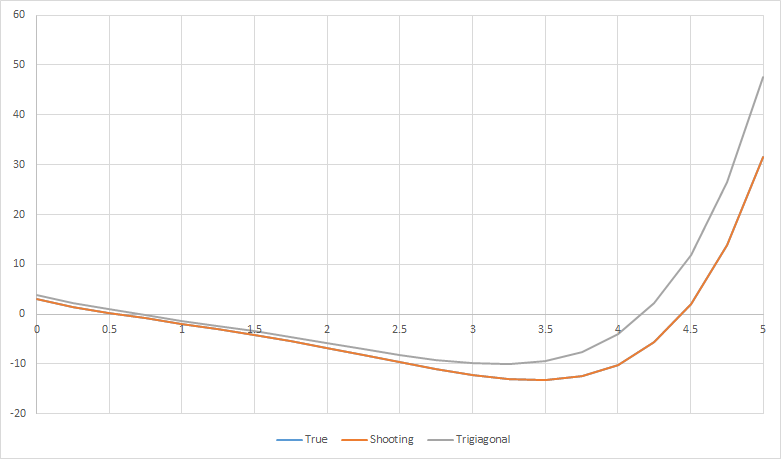
\includegraphics[width=0.9\linewidth]{pics/plot3.png}
		\caption{Шаг $h=0.25$}
	\end{subfigure}
	\begin{subfigure}{0.5\textwidth}
		\centering
		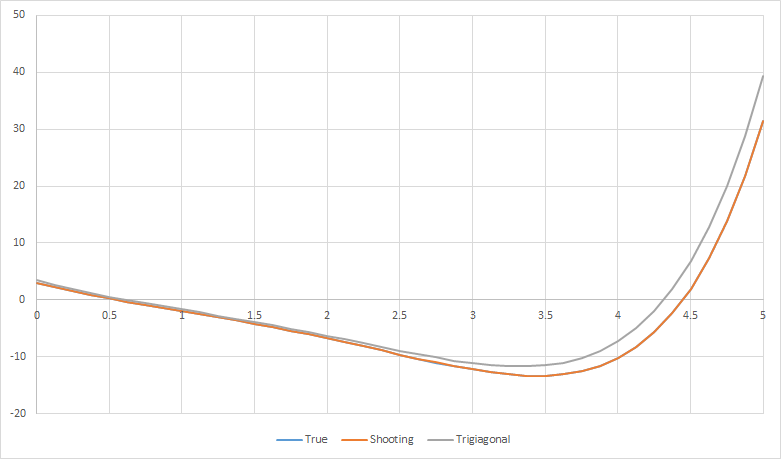
\includegraphics[width=0.9\linewidth]{pics/plot4.png}
		\caption{Шаг $h=0.125$}
	\end{subfigure}
	\caption{Графики численных решений}
\end{figure}

\begin{figure}[h]
	\begin{subfigure}{\textwidth}
		\centering
		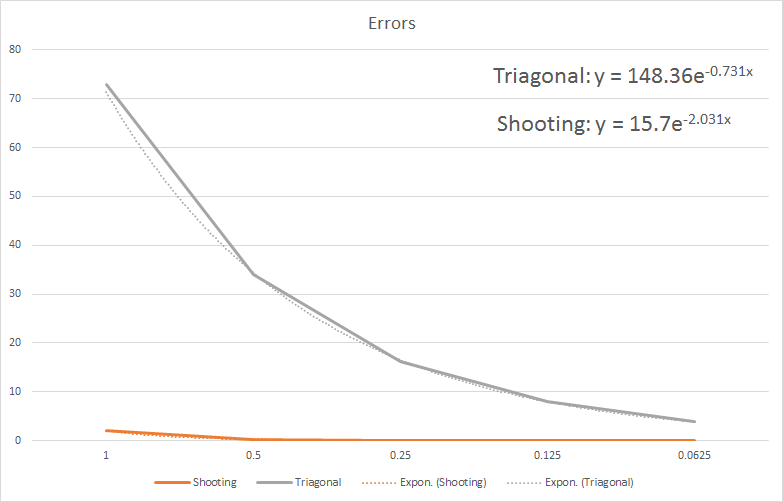
\includegraphics[width=0.6\linewidth]{pics/errors.png}
	\end{subfigure}
	\caption{График зависимости ошибки от размера шага}
\end{figure}

\pagebreak
\section{Выводы}

Как и ожидалось, метод прогонки оказался менее точным, и в плане роста ошибки и в плане скрытой константы. С другой стороны, метод стрельбы работат в несколько раз дольше (дополнительная степень точности во временной сложности решения на нахождение параметра), поэтому логично ожидать от него большей точности.

Как видно по графику зависимости ошибки от размера шага, у метода прогонки получилась ровно линейная зависимость от шага с большой константой, а у метода стрельбы более, чем квадратичная, как и ожидалось.

\end{document}
